%%%%%%%%%%%%%%%%%%%%%
% Short Sectioned Assignment
% LaTeX Template
% Version 1.0 (5/5/12)
%
% This template has been downloaded from:
% http://www.LaTeXTemplates.com
%
% Original author:
% Frits Wenneker (http://www.howtotex.com)
%
% License:
% CC BY-NC-SA 3.0 (http://creativecommons.org/licenses/by-nc-sa/3.0/)
%
%%%%%%%%%%%%%%%%%%%%%

%----------------------------------------------------------------------------------------
%	PACKAGES AND OTHER DOCUMENT CONFIGURATIONS
%----------------------------------------------------------------------------------------

\documentclass[paper=a4, fontsize=11pt]{scrartcl} % A4 paper and 11pt font size

\usepackage{graphicx}
\usepackage[T1]{fontenc} % Use 8-bit encoding that has 256 glyphs
\usepackage{fourier} % Use the Adobe Utopia font for the document - comment this line to return to the LaTeX default
\usepackage[english]{babel} % English language/hyphenation
\usepackage{amsmath,amsfonts,amsthm} % Math packages

\usepackage{lipsum} % Used for inserting dummy 'Lorem ipsum' text into the template

\usepackage{sectsty} % Allows customizing section commands
\allsectionsfont{\centering \normalfont\scshape} % Make all sections centered, the default font and small caps

\usepackage{fancyhdr} % Custom headers and footers
\pagestyle{fancyplain} % Makes all pages in the document conform to the custom headers and footers
\fancyhead{} % No page header - if you want one, create it in the same way as the footers below
\fancyfoot[L]{} % Empty left footer
\fancyfoot[C]{} % Empty center footer
\fancyfoot[R]{\thepage} % Page numbering for right footer
\renewcommand{\headrulewidth}{0pt} % Remove header underlines
\renewcommand{\footrulewidth}{0pt} % Remove footer underlines
\setlength{\headheight}{13.6pt} % Customize the height of the header

\numberwithin{equation}{section} % Number equations within sections (i.e. 1.1, 1.2, 2.1, 2.2 instead of 1, 2, 3, 4)
\numberwithin{figure}{section} % Number figures within sections (i.e. 1.1, 1.2, 2.1, 2.2 instead of 1, 2, 3, 4)
\numberwithin{table}{section} % Number tables within sections (i.e. 1.1, 1.2, 2.1, 2.2 instead of 1, 2, 3, 4)

\setlength\parindent{0pt} % Removes all indentation from paragraphs - comment this line for an assignment with lots of text

%----------------------------------------------------------------------------------------
%	TITLE SECTION
%----------------------------------------------------------------------------------------

\newcommand{\horrule}[1]{\rule{\linewidth}{#1}} % Create horizontal rule command with 1 argument of height

\title{	
\normalfont \normalsize 
\textsc{CS 472 Evolutionary Computation} \\ [25pt] % Your university, school and/or department name(s)
\horrule{0.5pt} \\[0.4cm] % Thin top horizontal rule
\huge Assignment 1b \\ % The assignment title
\horrule{2pt} \\[0.5cm] % Thick bottom horizontal rule
}

\author{Alex Cochrane} % Your name

\date{\normalsize\today} % Today's date or a custom date

\begin{document}

\maketitle % Print the title

%------------------------------------------------

%\horrule{0.5pt} \\[0.4cm] % Thin top horizontal rule
\section{Abstract}

%------------------------------------------------
\paragraph{} The problem for this project was to create a Genetic Algorithm(GA) for a set of benchmark optimization problems. My GA works as it is expected to but my populations rarely start with a good enough individual to ever get to a global minimum using hill-climbing. Introducing crossover had little affect at increasing the effectiveness of the GA. The results of the runs through the GA however show that conformation to the best solution is done in each case. In other words, the population might not move towards a global minimum but it does move towards the best individual and their local minimum.
%------------------------------------------------

\horrule{0.5pt} \\[0.4cm] % Thin top horizontal rule
\section{Algorithm Description}

%------------------------------------------------
\paragraph{} The algorithms used to create the GA revolve around tournament selection for a generational type. Below is some pseudo code for what will be explained next. To begin the GA that I built uses generational tournament selection. The pseudo code demonstrates that generations were built that then were used to replace the current population after crossover/mutation/etc. The fitness was measured during and after each generation was selected. The speed decrease was worth the assurance that the fitness values were always correct. After a new generation was created, crossover and mutation were preformed and the new generation replaced the population currently being stored.

\paragraph{} For crossover, there was a 50\% chance that I would swap a value in the vector of two side by side individuals in the new generation. Because elitism was not used and the new generation was not sorted yet, good and bad values could be swapped and better or worse solutions are almost guaranteed unless the same vector is being swapped.

\paragraph{} For mutation, there was a 25\% chance that I would subtract 0.01 from the value in the vector and a 25\% chance that I would add 0.01 to the value in the vector. There were also no restrictions on only accepting better solutions. If it wanted to accept worse values for the vectors it was more than capable of doing so.

\paragraph{} The fitness of each function is calculated on the benchmark functions provided for each one. It can be done solely for each individual for testing purposes if updated vector values have changed fitness and the value is needed now. The more common calculations for fitness were done for the whole population at once. After which, the population was then sorted by their fitness from minimum to maximum. This made print outs nicer and allowed me to "seed" my tournament selection to some degree, using some simple math to get values closer to 0 then 100.

\paragraph{} Some other information that is useful in recreating this GA is that populations consisted of 1000 individuals. They were filled with random values for their vectors. Runs consisted of 1000 generations or enough generations to get within a thousandth of 0.

\paragraph{Pseudo Code}
\begin{verbatim}
while ( Individual[]->fitness > 0.01 ) //larger then the smallest value measured
    if( repeated fitness 100 times || 1000 generations have been created)
        break
    while( next Population is not filled )
        create a new individual to put in the population
        randomly select an individual from the current population N = 5 times
        select the one with the best fitness and make the new individual it
    crossover
    mutate
    calculate the new fitness / sort
\end{verbatim}

\paragraph{}When the process is over it prints the best solutions fitness which should be below 0.01 unless it got stuck with a bad population that could not get to zero. It also prints how many times it iterated just to get a feel of how changes made the process more efficient or not. For most well situated solutions \~0 is found much sooner then the max 1000 generations.
%------------------------------------------------

\horrule{0.5pt} \\[0.4cm] % Thin top horizontal rule
\section{Results}

%------------------------------------------------

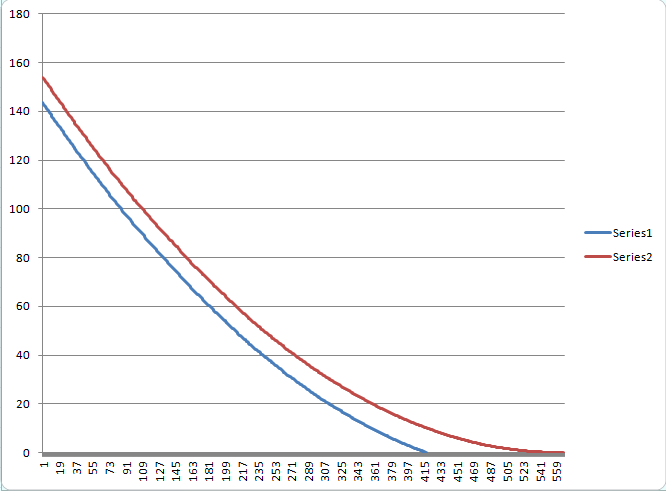
\includegraphics{Sphere}
Sphere Graph

\paragraph{} The following set of graphs will feature two lines, one showing best individual fitness and then an average individual fitness over the total duration of the run. The first graph is of the sphere function. The red line here represents the average fitness for the population. The blue line is representing that of the best individual. In this instance, a very good solution was in the initial population but during tournament selection, it was not chosen with great bias and therefore the population was slow to converse on it.

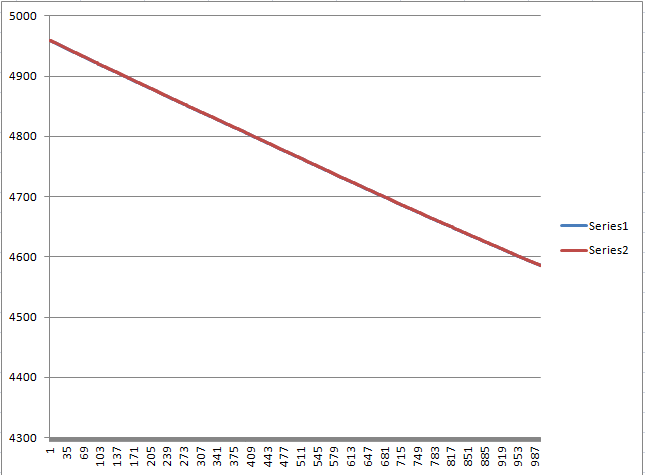
\includegraphics{Schwefel}
Schwefel Graph 

\paragraph{} This graph is for the Schwefel function. The red line represents the average, the blue line would represent the best case but because this graph is standardized the line is really hard to see. The graph itself has the correct slope that you would expect with a steep initial reading and then steadying off into a gradual decent. The initial slope however is small and as this graph shows very well, the population becomes more and more centralized to the best individual as it hill climbs down into a valley.

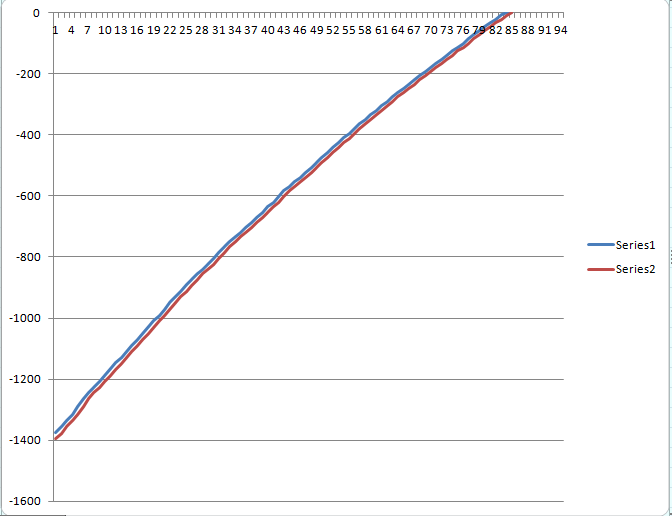
\includegraphics{Rosenbrock}
Rosenbrock Graph

\paragraph{} With the Rosenbrock graph, the blue line shows the best individual while the red line shows the average. Rosenbrock has the fitness function that produces negative values. This was handled in code by taking the absolute value but I thought the real graph would look unique. For this graph a lot of movement can be seen by the slope of the lines. While it is not clear in the graph, the values themselves make a drastic junk from bad values to conform quickly to the best individual.

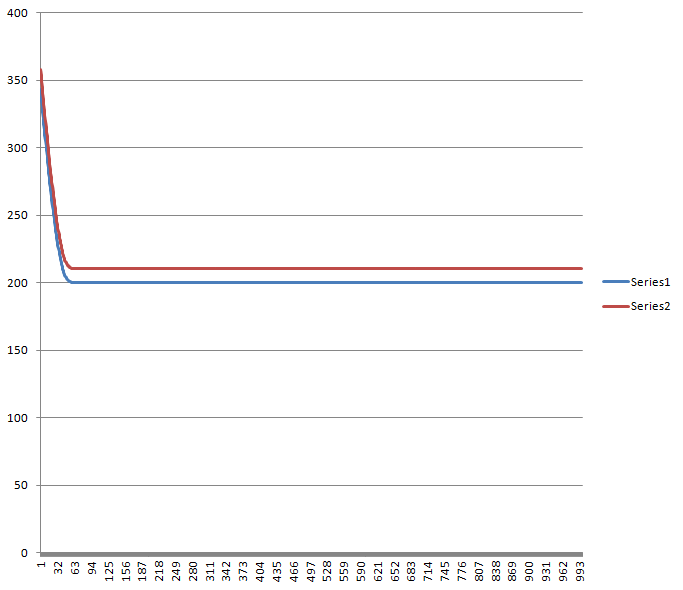
\includegraphics{Rastrigin}
Rastrigin Graph

\paragraph{} Finally with the Rastrigin graph the drastic curve can be seen. The blue line representing the best individual moves quickly into a hole that it cannot leave while at almost the same speed the entire population, represented by the red line, moves towards a stagnant state as well. This steep initial movement is present in all the graphs but it is masked by the linear nature of the graphs and their axes morphing.

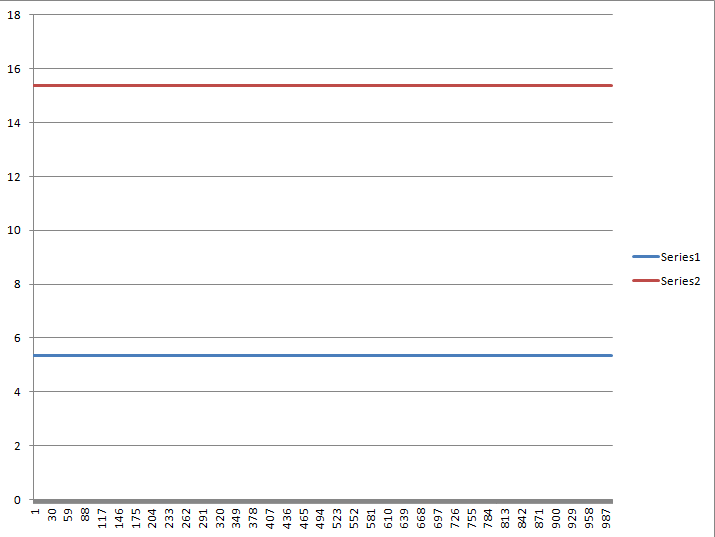
\includegraphics{Ackley}
Ackley Graph

\paragraph{} The Ackley graph is interesting in the since that the individuals fitness values are not changing. This is because drastic changes in vector values are needed to get to the function to produce different values for fitness. Therefore the fitness gets stuck in the hole that it falls into at the start. The exponential nature of the fitness function creates this uniqueness.

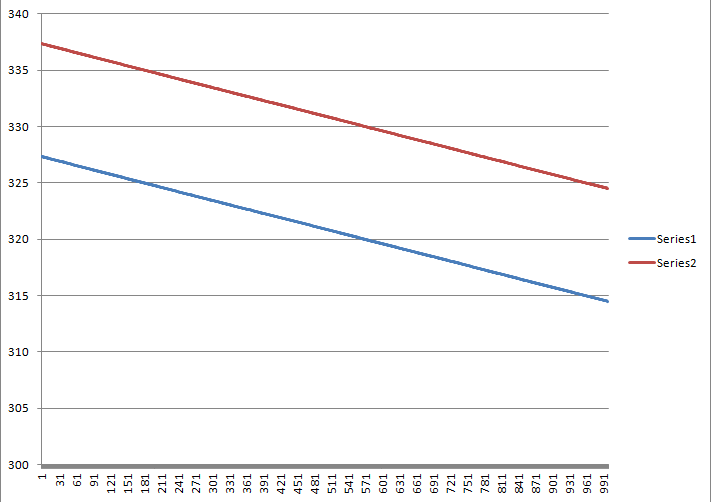
\includegraphics{Griewangk}
Griewangk Graph

\paragraph{} For this graph it is easy to see that the fitness is slowly moving towards the minimum. The average fitness stays at an almost constant distance away from the best fitness. The population has varying fitnesses but the average seems to stay very linear. With more time or a larger interval the same hole is found.

%------------------------------------------------

\horrule{0.5pt} \\[0.4cm] % Thin top horizontal rule
\section{Conclusion}

%------------------------------------------------
\paragraph{} The Genetic Algorithm seems to be working well in the since that it is taking good individuals and mutating them along with crossover to get a better next generation. The problem with this solution however is that a great individual is not present in the population at the start. Without this individual that is almost at the minimum at the start, it is very unlikely to actually find the global minimum.

\paragraph{} Some improvements that could have been done were to add an individual to the population that was not random but was in fact very close to the actual minimums vector/fitness. This would guarantee that I had an individual that would be able to move to the minimum. This does take away from the whole purpose of the GA but as stated before, it guarantees a solution is found.

\paragraph{} While it would be interesting to get these problems to all work correctly, the run time for them with 1000 individuals in the population takes quite some time. Each fix could take up to 5 minutes to run that fix to see if an improvement was made. Therefore I would like to rewrite the way I do sorting a bit but as just an exercise I have learned quite a bit about GA's and how they operate.
%------------------------------------------------

\horrule{0.5pt} \\[0.4cm] % Thin top horizontal rule
\end{document}
